\documentclass[11pt]{article}
\renewcommand{\baselinestretch}{1.1}
\setlength{\parindent}{0cm}

%%% Add packages here
	\usepackage{graphics}
	\usepackage{graphicx}
	\usepackage{lscape}
	\usepackage{amsfonts}
	\usepackage{amsmath}
	\usepackage{amsthm}
    \usepackage{array}
	\usepackage{amssymb}
	\usepackage{latexsym}
	\usepackage{verbatim}
    \usepackage{color}
	\usepackage{fancyhdr}
	\usepackage{fancybox}
    \usepackage{mathtools}
    \usepackage{subcaption}
	\usepackage[colorlinks]{hyperref}
 %   \usepackage{times}
 %   \usepackage{w-thm}
%    \usepackage[authoryear]{natbib}
    \usepackage{float}
    \usepackage[utf8]{inputenc}
    \usepackage[english]{babel}
    \usepackage{multicol}
%%%%%%%%%%%%%%%%%%%%%%%%%%%%%%%%%%%%%

%%% Margins
\addtolength{\oddsidemargin}{-.50in}
\addtolength{\evensidemargin}{-.50in}
\addtolength{\textwidth}{1.0in}
\addtolength{\topmargin}{-.40in}
\addtolength{\textheight}{0.80in}

%%% Header
	\pagestyle{fancy}
	\chead{\groupname}
	\rhead{}
	\lhead{}
	\cfoot{\thepage}
	\renewcommand{\headrulewidth}{0.4pt}
%%%%%%%%%%%%%%%%%%%%%%%%%%%%%%%%%%%%%


%%%%%%%%%%%%%%%%%%%%%%%%%%%%%%%%%%%%%%%%%%%%%%%%%%%%%%%%%%%%%%%%%%%%%%%%%%
%%%%%%%%%%%%%%%%%%%%%%%%%%%%%%%%%%%%%%%%%%%%%%%%%%%%%%%%%%%%%%%%%%%%%%%%%%
%%%%%%%%%%%%%%%%%%%%%%%%%%%%%%%%%%%%%%%%%%%%%%%%%%%%%%%%%%%%%%%%%%%%%%%%%%
%%%%%%%%%%%%%%%%%%%%%%%%%%%%%%%%%%%%%%%%%%%%%%%%%%%%%%%%%%%%%%%%%%%%%%%%%%
%%% START MAKING CHANGES HERE!

%%% Group details - PLEASE PUT YOUR GROUP NUMBER HERE!
\newcommand{\groupname}{Longitudinal Data Analysis (2016--2017)}
%%%%%%%%%%%%%%%%%%%%%%%%%%%%%%%%%%%%%

\begin{document}
\clearpage\thispagestyle{empty}

\begin{center}
	% title
	\textbf{\huge{Factors Influencing Evolution of Haematocrit Level in Renal Graft Patients}} \\[1.7cm]
	% details
	\Large{
	Longitudinal Data Analysis \\
	2016-2017 \\[0.5cm]
	$2^{nd}$ year Master of Statistics \\
	Hasselt University	
	}
\end{center}

\vspace*{1cm}
\textbf{\large{Group members:}}\\
Ezgi Tanriver Ayder (1541821) \\
Oana Petrof (1541809) \\
Olusoji Oluwafemi Daniel (1541893) \\
Owokotomo Olajumoke Evangelina (1539654) \\[0.5cm]

\noindent\textit{Submission Date:} 28/10/2016

\vspace*{3cm}
\textbf{\large{Lecturers:}}\\
Prof. Dr. Molenberghs Geert  \\
Prof. Dr.  Verberke Geert


%%% THE WRITTEN PROJECT - MAX. 20 PAGES (everything included)
%%% page numbering starts here.
\newpage \setcounter{page}{1}

\begin{abstract}
\noindent\textbf{Background}: \\
Renal transplantation is a better alternative than dialysis for a patient with end stage renal disease. Several factors relating to patients are known to influence haemotocrit level of such factors. One of such factor is gender, which has been established that males have an acute rejection rate. To  better understand the evolution of haemotocrit level in renal graft patients, measurements are  taken repeatedly on these patients. Repeated measures are obtained when a response is measured repeatedly on a subject. Modelling these response changes over time is often of primary interest and as such, methods that disentangle the within subject variability and between subject variability need to be used.\\
\noindent\textbf{Objectives}:  \\
A longitudinal study of 1160 Renal graft patients, whose haematocrit level was observed over time is used to understand the evolution of haematocrit level over time. This study also investigates if Haematocrit level is affected by some important factors.\\
\noindent\textbf{Methodology}:  \\
Multivariate regression method is used to model haematocrit evolution over time while accounting for the correlation within subjects and also correcting for factors of interest. A two stage analysis and a linear mixed model is used as a more general and broad method to model the evolution of interest. Results from this three modelling approach are also contrasted %However, a drawback of 2 stage analysis is that it can not be applied in a situation of a subject with one measurement. Thus A more parsimonious model is sought for in order to increase efficiency in making inference about the mean parameter using the likelihood ratio test and contrast is used to answer the primary question of interest.\\
\noindent\textbf{Results}:   \\
Results obtained showed that the evolution of haematocrit over time for males is different from females, however there is no difference in the evolution of haematocrit levels between patients, who rejected the transplant and who did not. Similarly, no difference is observed in the evolution of Haematocrit levels for the patients with history of cardiovascular disease and those without the history of cardiovascular disease.
The results from the linear mixed model are almost consistent with the ones obtained in the multivariate regression.\\
\noindent\textbf{Conclusions}:  \\
The analysis conducted was consistent with other past studies in terms of the findings about the influence of gender on the haematocrit level. The three models show that the patient's cardiovascular problems 
are not influenced by the haematocrit level. Multivariate regression model and 2 stage analysis model did not find a significant result in terms of the renal transplant rejection while the linear mixed model indicate a borderline situation.

\noindent\textit{Key Words}: Renal Graft, Haematocrit, Multivariate Regression, 2 Stage Analysis, Linear Mixed Model.

\end{abstract}
\rule{\textwidth}{0.4pt}

\section{Introduction}\label{introduction}


Renal graft is a well known therapeutic intervention for patients, who are in need of renal replacement therapy or suffers from serious renal impairment. The outcomes of this transplantation are influenced by many variables such as donor age; as the older the age of a donor, it is more likely to see rejection symptoms or other adverse effects on the function of the transplant and long term outcomes \cite{bib1}. Successful kidney graft provides increased quality of life and is more economically and medically efficient than long term dialysis treatment. In order to make a foreseen prediction on possible rejection of renal transplant, Haematocrit levels could be considered. Haematocrit is a test that is used to measure the proportion of red blood cells in the blood, which carry oxygen throughout the body \cite{bib4}. The amount of the red blood cells in the body could indicate certain diseases.\\

\noindent High Haematocrit implies that considering the age and sex effects, percentage of red blood cells in the blood is above the indicated upper limits of a normal person \cite{bib2}. It is also observed that increased risk of cardiovascular events in patient history causes high Haematocrit values \cite{bib3}. However, the effect of cardiovascular disease events on Haematocrit seems to differ for distinct age groups and by gender. Gender has an effect here as it is noted that although there was no decrease risk of cardiovascular disease in men with lower than median Haematocrit values, women was observed to show increased risk of cardiovascular events with lower Haematocrit values. Elevated Haematocrit values are also frequently observed as a result of complication after renal transplantation, especially during the first three to six months \cite{bib9}. \\

This report is organized as follows: Section 1 describes the study objective and data structure while section 2 provides information on the statistical methods and models that are used to analyze the data. Section 3 presents the results on the exploratory data analysis and statistical analyses, such as Multivariate Regression, 2 Stage Analysis and Linear Mixed Model while also providing discussion on the obtained results from the analysis. Lastly, section 4 presents the discussion of findings from the result. 


\subsection{Objective of the Study} 
The aim of this study is to observe the evolution of Haematocrit over time and the impact of gender and age. It is also of interest to investigate if this evolution is affected by cardiovascular problems that was experienced in the past or by the occurrence of rejection symptoms during the first three months after the transplantation was conducted. 

\subsection{Data Description}

The dataset for this study is from a longitudinal study in which Hematocrit measurement were taken over 1160 subjects with the total of 13920 observations over a period of 10 years. Other variables also measured are described as follows:
\begin{itemize}
\item  ID: identification number for every patient
\item  MALE: represents the gender of the patients, where 0=female and 1=male
\item  AGE: represents age at transplantation
\item CARDIO: indicates if the patient experienced a cardio-vascular problem during the years
preceding the transplantation and is represented by  0=no and 1=yes
\item  REJECT: shows if the patient shown symptoms of graft rejection during the first three
months after the transplantation with 0=no and 1=yes
\item  Hc0: Haematocrit level at moment of transplantation
\item  Hc06: Haematocrit level 6 months after transplantation
\item  Hc1 - HC10: Haematocrit level for 1 year, 2 year,..., 10 years after transplantation
\end{itemize}

\noindent There are in total of 494 females and 666 males, ages between 15 and 76 years, followed at the moment of transplantation, six months after and once in every year for 10 years. 367 patients in total were observed to reject the transplant at time point 0. Haematocrit level were measured at fixed time point with number of measurement differing from one patient to the other. Although the time points in which Haematocrit level was measured is fixed, these time points are not equally spaced essentially because of the measurement taken at 6 months and there were missing Haematocrit measurements. In other words, the design of the study that produces the dataset is balanced but the resulting dataset is unbalanced due to missingness and unequally spaced time points.


\section{Methodology}

\noindent  Over the years several methods have been proposed for the analysis of longitudinal data to study evolution of subjects over time. While early techniques applied normal known methods to this kind of data, they totally ignore the correlation within subjects because of repeated measurements taken on a subject. To take into account this correlation within subjects methods such as; analysis at each time point separately, analysis of area under the curve, analysis of endpoint, analysis of increments and Analysis of Covariance \cite{bib8} were proposed. These are referred to as simple method and thus solve the correlation problem but give a partial view of the problem, hence there is need for models that use all information in these kind of datasets. Such models will be considered in this study to prevent analysis of partial information. In other words, methods used in this study uses all the information contained in the dataset, although these methods have some shortcomings.

\subsection{Multivariate Regression}

In order to study the evolution of Haematocrit over time and how this evolution depends on Gender, Age, Cardio and Reject, a multivariate regression model was fit. Likelihood ratio test ($G^2$) was used in order to obtain the most parsimonious model that describes the average evolution of Haematocrit over time by comparing the saturated model with the reduced model, taking out one covariate at a time.

\noindent Let $Y_i$ be the vector of repeated measurements for the subject i, such that  $Y_i$= $(Y_{i1} Y_{i2} \ldots Y_{in} )^{'}$. The general multivariate model assumes that $Y_i$ satisfies regression model as follows:
\begin{equation}\label{model1}
Y_{i}=X_{i}\beta_{i}+\epsilon_{i}
\end{equation}
with 
\[ \begin{dcases*} X_{i}: & matrix of covariates\\ 
\beta_{i}: & vector of regression parameters \\ 
\epsilon_{i}:  &  vector of error components 
\end{dcases*}  \]

where $\epsilon_{i} \sim N(0,\Sigma)$. \\

\noindent $X_{i}$ is the matrix of covariates male,age,cardio,reject, time, interaction between each of these variable with time and possibly higher powers of time. The mean structure $X_{i}\beta_{i}$ is modeled similar to classical linear regression and ANOVA models. $\Sigma$ is a general (n x n) covariance matrix. The design of the ranal transplant dataset is a balanced design since fixed time points are observed for each patient. However,the dataset could be also considered as unbalanced due to the missing observations for different Haematocrit levels and unequally spaced time points for each measurement. Looking at the variance-covariance matrix, the data should be correlated as several measurements are taken on the same patient at different time points
and it will be explored in the analysis takeing into account the design of the experiment.


\subsection{Two Stage Analysis}
Two stage model formulation is considered due to the unequal number of measurements per subject and the unequally spaced time points of the measurements. Therefore, multivariate regression techniques are often not applicable and subject specific profiles over time could be well approximated by linear regression functions. Therefore,   two stage analysis is conducted in order to see subject specific effect of covariates on the response\cite{bib8}.

\subsubsection*{Stage 1}

\noindent Let the response vector $Y_{i}$ for the $i^{th}$ subject be $Y_i$= $(Y_{i1} Y_{i2} ... Y_{in} )^{'}$. The response $Y_{ij}$ for $i^{th}$ subject, measured at time $t_{ij}$, i=1,..,1160, j=1,..,10 is given by as follows:
\begin{equation}\label{model2}
Y_{i}=Z_{i}\beta_{i} + \epsilon_{i}
\end{equation}
where;
\[ Z_{i} = \begin{pmatrix} 1 & t_{i1} & t_{i1}^2 \\  1 & t_{i2} & t_{i2}^2 \\ \vdots & \vdots  & \vdots \\ 1 & t_{in_{i}} & t_{in_{i}}^2  \end{pmatrix} \]

\begin{equation}\label{model3}
Y_{ij}=\beta_{1i}+\beta_{2i}t_{ij}+\beta_{3i}t_{ij}^2+\epsilon_{ij}
\end{equation}
Parameters $\beta_{1i}$, $\beta_{2i}$ $\beta_{3i}$ are the unknown subject specific regression coefficients and $\epsilon_{ij}$ explains the within subject variability where $\epsilon_{i} \sim N(0,\Sigma)$. In order to extend stage 1 model, $F_{meta}$ test is conducted to investigate whether quadratic or cubic time effect should be added to the model. Furthermore, the overall coefficient $R^{2}_{meta}$ of multiple determination is obtained to investigate the total variability within subjects explained by the considered model.

\subsubsection*{Stage 2}
In stage 2 between subject variability is explored by relating the $\beta_{i}$ to known covariates. 
\begin{equation}\label{model4}
\beta_{i}=K_{i}\beta+ b_{i}
\end{equation}
where 
$K_{i}$ is a (3 x 5) matrix of known covariates. $\beta$ is a 5 dimensional vector of unknown regression parameters and $b_{i} \sim N(0,D)$.\\
\[ \begin{dcases*} \beta_{1i} = \beta_{1} + \beta_{2}Male_{i} + \beta_{3}Age_{i} + \beta_{4}Cardio_{i} + \beta_{5}Reject_{i}+ b_{1i},\\ 
\beta_{2i} = \beta_{6}Male_{i} + \beta_{7}Age_{i} + \beta_{8}Cardio_{i} + \beta_{9}Reject_{i}+ b_{2i},\\
\beta_{3i} =  \beta_{10}Male_{i} + \beta_{11}Age_{i} + \beta_{12}Cardio_{i} + \beta_{13}Reject_{i}+ b_{3i}\\
\end{dcases*}  \]

 \[ Male_{i} = \begin{dcases*} 1 & if male \\ 
0 & female\\ \end{dcases*}  \]
 \[ Cardio_{i} = \begin{dcases*} 1 & if yes \\ 
0 & no\\ \end{dcases*}  \]
\[ Reject_{i} = \begin{dcases*} 1 & if yes \\ 
0 & no\\ \end{dcases*}  \]

\noindent Parameter $b_{1i}$ indicates how much the subject specific intercept deviates from the average intercept $\beta_{1}$. Parameter $b_{2i}$ expresses how much the subject specific slope for subject i deviates from the linear average slope  $\beta_{6},\beta_{7},\beta_{8}$ and $\beta_{9}$. Parameter $b_{3i}$ indicates how much the subject specific slope for subject i deviates from the quadratic average slope  $\beta_{10},\beta_{11},\beta_{12}$ and $\beta_{13}$. Therefore,$b_{1i}$, $b_{2i}$ and $b_{3i}$ include some unexplained between variability. The random effects are assumed to follow a normal distribution with mean vector zero and covariance matrix D ($b_{i} \sim N(0,D)$). The second stage in this case is a weighted analysis where the standard errors of the estimated $\beta 's$ in the first stage are used as weights.

\subsection{Linear Mixed Model}
The 2 stage analysis above random variability is introduced by replacing the the $\beta_{i}$ by their estimates $\hat{\beta_{i}}$ also number of measurement available by each subject and the time point which measurement were taken which the covariance matrix of $\beta_{i}$ highly depends on have not been taken into account in which the linear mixed model will address\cite{bib8}.

A random-effect model or linear mixed model corresponding to the two-stage model can be considered to obtain more precise estimates of the regression coefficients by taken into account the correlations among the measurements by combining the 2 stage models into one model\cite{bib8}.
\[ \begin{dcases*} Y_{i} = X_{i}\beta_{i} + Z_{i}b_{i} +\epsilon_{i} \\ 
b_{i} \sim N(0,D),\\
\epsilon_{i} \sim N(0,\Sigma_{i}),\\
b_{1},....,b_{n},\epsilon_{1},.....\epsilon_{n} independent\\
\end{dcases*}  \]


\begin{eqnarray}\label{model5}
\nonumber Y_{ij} &=& \beta_{1}Male_{i} + \beta_{2}Age_{i} + \beta_{3}Cardio_{i} + \beta_{4}Reject_{i}\\
\nonumber &+& (\beta_{5}Male_{i} + \beta_{6}Age_{i} + \nonumber \beta_{7}Cardio_{i} + \beta_{8}Reject_{i})t_{ij}\\
\nonumber &+& (\beta_{9}Male_{i} + \beta_{10}Age_{i} + \beta_{11}Cardio_{i} + \beta_{12}Reject_{i})t^{2}_{ij}\\
 &+& b_{1i} + b_{2i}t_{ij} + b_{3i}t_{ij}^2
+ \epsilon_{ij}
\end{eqnarray}

From this model, it can be said that the $\beta_{1}$ represents the average intercept. Furthermore, $b_{1i}$, $b_{2i}$ and $b_{3i}$ represent the subject-specific random intercept, linear slope and quadratic slope respectively. $\beta_{i}$ is a 12 dimensional vector containing the fixed effects, $b_{i}$ is the 3 dimensional vector containing the random effects, and $\epsilon_{i}$ is an 1160 dimensional vector of residual component. The D (3 x 3) covariance matrix represents the random effect correlations and the $\Sigma_{i}$ covariance matrix contains the measurements error.

\subsection{Softwares}
SAS 9.4\cite{bib7} and R\cite{bib6} were used in order to conduct the statistical analysis and graphical illustrations.

\section{Results \& Discussion}
In this section, the results of the exploration and analysis of the data is presented alongside discussions as regards findings in relation to the objective of the study. A key advantage of the dataset under consideration is the fixed time point in which measurements were measured but a feature to worry about is not only the missingness in the dataset but also the unequally spaced time points in which measurements were taken. 

\subsection{Exploratory Analysis}
While major characteristics of the data has already been discussed in previous sections, it is also of interest to have a better understanding of the data. A total of 1159 patients have their Haematocrit level measured at baseline and the only time point where all 1160 patients were measured was at 6 months after renal graft. Also it was observed that number of patients measured at every time point after 6 months continues to decline (with only 348 patients present for the last measurement) indicating dropout of patients from this study (see table 1 below). 

\begin{table}[H]
\centering
\begin{tabular}{cccc}
  \hline
Time(years) & Average & Variance & Number of Patients \\ 
  \hline
0.00 & 31.86 & 36.85 & 1159 \\ 
0.50 & 38.83 & 31.15 & 1160 \\ 
1.00 & 39.71 & 34.61 & 1159 \\ 
2.00 & 39.70 & 30.30 & 1073 \\ 
3.00 & 39.17 & 29.06 & 955 \\ 
4.00 & 39.16 & 30.31 & 846 \\ 
5.00 & 39.02 & 29.80 & 742 \\ 
6.00 & 39.11 & 26.87 & 652 \\ 
7.00 & 38.85 & 31.37 & 565 \\ 
8.00 & 38.35 & 28.46 & 488 \\ 
9.00 & 38.57 & 29.11 & 411 \\ 
10.00 & 38.49 & 27.62 & 348 \\ 
   \hline
\end{tabular}
\caption{General Summaries}
\end{table}

\noindent While the number of patients measured at every time point continue to dwindle as the study progresses, the mean Haematocrit remained constant (approximately 39) from 6 months onward. The variance of these measurements was also largest at baseline and continue to generally decrease with time but remain approximately close to each other. These suggests that the evolution of Haematocrit was really different at baseline compared to other time points and possibly any notable change in evolution of Haematocrit level occurred between baseline and 6 months after the surgery. This is typical with treatments involving organ transplant as it is expected that the body rejects the new organ with a space of 6 months after surgery.  \\

\noindent Of the 1160 patients, only 339 patients had full measurements, i.e. measured at all time points, 68 patients missed the last measurement and had no measurement for the $10^{th}$ year. A total of 73 patients missed the last two measurements and a total of 86 patients missed the last four measurements. In summary, there seems to be no definite pattern to missingness in this dataset as there are 19 unique missingness patterns but this will be ignored for subsequent analysis (see table in appendix).

\subsubsection{Individual Profile}
\noindent The interest in longitudinal analysis is the evolution of individual patients over time, this does not only give an idea about the most appropriate subject specific regression but also provides an idea of the variability between and within subjects under study.

\begin{figure}[H]
\centering
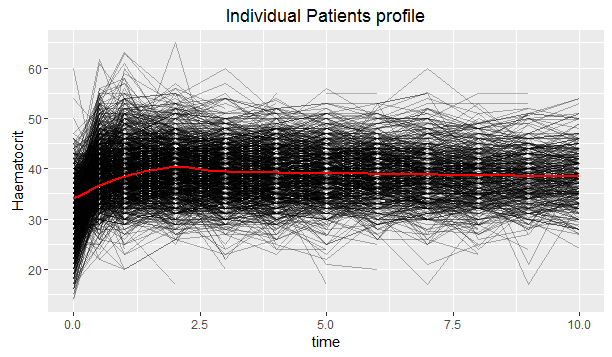
\includegraphics[scale=0.8]{patientsprofile.png}
\caption{Patients Profile}
\end{figure}

The profile plot above reveals the classical observation inherent to most longitudinal studies. There is much variability between patients than within patients and most patient saw an increase in their Haematocrit level between baseline and six months (see figure 1). A look at the patients profile across gender strata reveals that males tend to have higher profiles than females indicating a possible difference in evolution of Haematocrit levels of males to females (see figure 8 in appendix). On the other hand, no unique evolution pattern for both patients with or without previous cardio-vascular problems if the profiles are checked based on history of cardio-vascular problems before transplantation (see figure 10 in appendix). The same pattern is observed for the patients who suffered and did not suffer from a rejection of the transplant after 3 months as it can be seen in the figure 9in the appendix. 
Therefore, there is need to consider random intercepts and slopes as clearly the evolution of these patient differs.

\subsubsection{Mean Structure}
Of interest in longitudinal data analysis is the average evolution of the response (Haematocrit level in this case) over time. This gives an idea of the marginal relationship between time and the response of interest.

\begin{figure}[H]
\centering
\begin{minipage}{.5\textwidth}
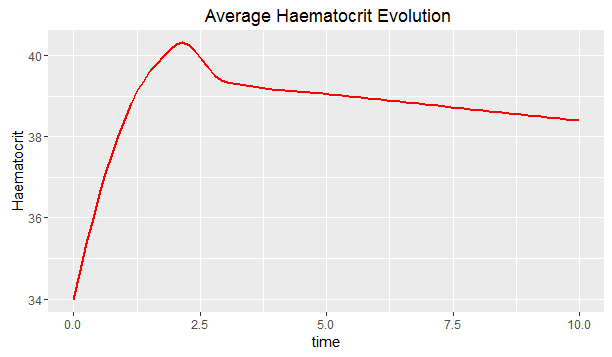
\includegraphics[scale=0.6]{averageevolution.png}
\caption{Average Evolution Loess}
\end{minipage}
%\hfill
\begin{minipage}{.4\textwidth}
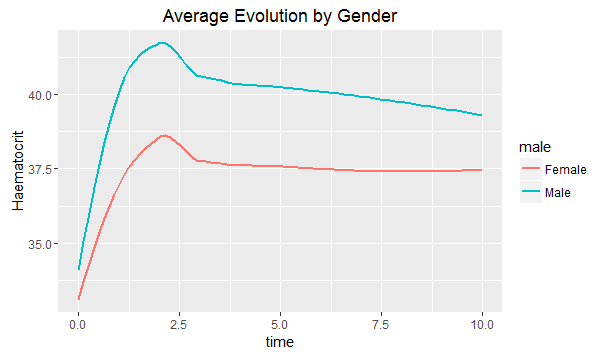
\includegraphics[scale=0.6]{averageevolutiongender.png}
\caption{Average at Time Points}
\end{minipage}
\end{figure}

Figure 2(time as continuous) presents the average evolution over time. It is observed that on the average, the relationship between time and Haematocrit level is quadratic. Once again, the baseline average Haematocrit level appears to differ from the rest distinctively (see figure 2). A look at the average level across gender corroborates what was observed when exploring individual patients profile. Male patients evolve higher than female patients and males tend to start high on the average (see figure 3). Furthermore, history of cardio-vascular problems seem not to influence the evolution of Haematocrit level but graft rejection plays the other way as it is observed that the evolution of patients with graft rejection is lower on average compared to those without graft rejection within the first three months. Importantly, the quadratic evolution of Haematocrit level in time was observed in all groups, which is an indication not to go for models beyond quadratic function of time at the marginal level.

\subsubsection{Variance Structure}
To get an understanding of the variance function over time, a boxplot of the variance of measurements taken at each time point is plotted (time treated as discrete) and also a smooth function of the residuals obtained from exploration of the mean structure is considered.

\begin{figure}[H]
\centering
\begin{minipage}{.5\textwidth}
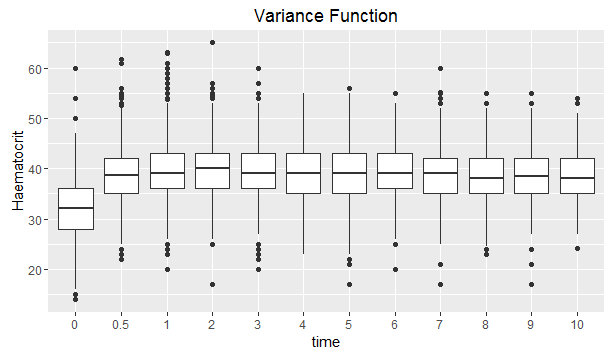
\includegraphics[scale=0.5]{variancefunction.png}
\caption{Variance Function}
\end{minipage}
%\hfill
\begin{minipage}{.4\textwidth}
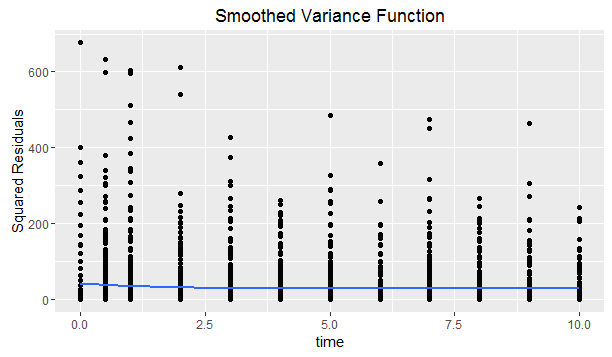
\includegraphics[scale=0.5]{variancefunction2.png}
\caption{Variance Function Smooth}
\end{minipage}
\end{figure}

Both figures suggest variance in Haematocrit measurements remained relatively constant from the third measurement onward (see figure 4 and 5) and slight curvature was observed in the smooth function between baseline and the third measurement suggesting that the variance is a quadratic function of time. Also, it is observed that Haematocrit measurements taken at baseline is quite different from those taken at other time points. 

\subsubsection{Correlation Structure}
In terms of correlation between Haematocrit measurements at different time points, it was observed that two successive measurements are more correlated than measurements taken at other time points. It was also observed that the correlation between these measurements decreases as the differences in time increases (see figure 13 in appendix).

\subsubsection{Subject Specific Regression}
Essential to mixed model methodology in longitudinal setting is a functional relationship between the response of interest and time at the subject level. To select the best possible regression relation between Haematocrit level and time, a linear relationship and a quadratic relationship was assumed and examined between time and Haematocrit level. Each model was fitted for each subject and the results were combined in a form of meta-analysis using $R^{2}_{meta}$ and $F_{meta}$ as specified in \cite{bib2}.\\

The computed $R^{2}_{meta}$ for the assumed linear relationship is 0.234 while that of quadratic relationship is 0.31. While it is easy to conclude that a quadratic relationship is better, the known drawback of $R^2$ is also present here, in other words, $R^{2}_{meta}$ will always increase as higher order of time is added to the model, hence a meta-analysis form of the partial F-test in classical linear regression is used to ascertain if a quadratic relationship is better.

\begin{figure}[H]
\centering
\begin{minipage}{0.4\textwidth}
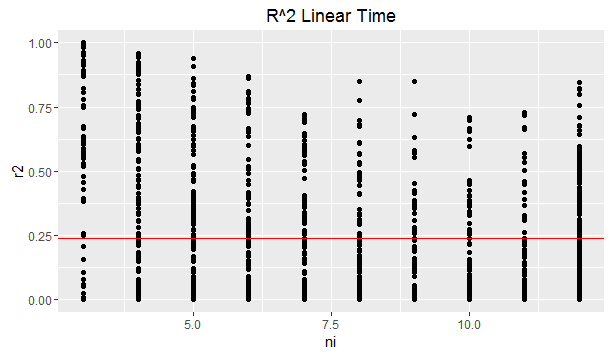
\includegraphics[scale=0.5]{r2meta.png}
\caption{$R^2_{meta}$ of Linear Time}
\end{minipage}
%\hfill
\begin{minipage}{0.5\textwidth}
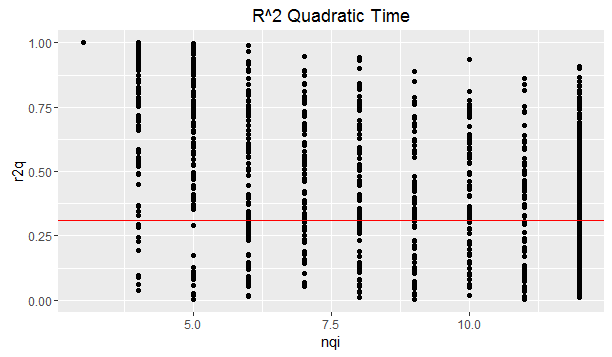
\includegraphics[scale=0.5]{r2metaquad.png}
\caption{$R^2_{meta}$ of Quadratic Time}
\end{minipage}

\end{figure}

The computed $F_{meta}$ is  2.412 with a p-value of 0.000 (compared with $F_{957,5961}$) which confirms that a quadratic function of time is needed in the subject specific regression.

\subsection{Multivariate Regression}
Based on findings from data exploration, multivariate regression model \ref{model1} as specified in previous section is fitted with $time^2$ as a higher power of time, also, interactions between covariate under study and time is considered, as these are of main interest to the study. The model is then reduced via likelihood ratio test\footnote{All estimates reported are based on Maximum Likelihood and unstructured variance covariance matrix} as discussed in the methods section.

\begin{table}[H]
\centering
\begin{tabular}{ccccccc}
\hline
Ref & Model & -2loglike & $G^2$ & pvalue & ParDiff & Removed\\
\hline
 & 1 & 54648.1 &  & & \\
1 & 2 & 54648.8 & 0.7 & 0.4 & 1 & $Cardio*time^2$\\
2 & 3 & 54650.3 & 2.2 & 0.13 & 1 & $reject*time^2$\\
3 & 4 & 54650.9 & 0.6 & 0.44 & 1 & $Age*time^2$\\
4 & 5 & 54654.9 & 4.00 & 0.046 & 1 & $male*time^2$\\
\hline
\end{tabular}
\caption{LR-Test for Reduction of Assumed Mean Structure}
\end{table}

From the table above, it can be deduced that one can easily assume same quadratic evolution for patients with history of cardio-vascular problems and those without history of cardio-vascular problem, also same can be said of patients who developed rejection symptoms during first 3 months after transplantation and those who did not. This position is however not the same in terms of gender of patients. Further likelihood ratio test showed that cardio*time, reject*time (which implies that the same linear slope can be assumed for each group) can be removed but these parameters are essential to the research question, hence they are retained in the model and tested via a contrast. Essentially, the final multivariate regression model is of the form;

\begin{eqnarray*}
Haematocrit_{ij} &=& \beta_{1}male_{i} + \beta_{2}cardio_{i} + \beta_{3}reject_{i} + \beta_{4}age_{i} + \beta_{7}male_{i}*time_{ij} \\
&+& \beta_{8}cardio_{i}*time_{ij} + \beta_{9}reject_{i}*time_{ij} + \beta_{10}Age_{i}*time_{ij} \\
&+& \beta_{11}male_{i}*time_{ij}^2 + \epsilon_{ij}
\end{eqnarray*}

In terms of covariance and correlation structure, plausible covariance structure for the $\Sigma$ matrix are toeplitz and AR variants but the study design does not support these structures as the measurements were not taken at equally spaced time intervals, hence the variance-covariance matrix and consequently the correlation matrix is left unstructured.

\begin{table}[H]
\centering
\begin{tabular}{ccccc}
\hline
Constrast & $\chi^2$ & F value & $Pr > \chi^2$ & $Pr > F$ \\
\hline
Evolution of Males vs Females & 98.32 & 32.77 & $<.0001$ &  $ <.0001$ \\
Evolution of Cardio vs No Cardio & 2.40 & 1.20& 0.3008 &  0.3013  \\
Evolution of Reject vs No Reject & 2.65 & 1.33& 0.2655 &0.2661  \\
\hline
\end{tabular}
\caption{Evolution of Gender, Cardio and Reject (Multivariate Regression)}
\end{table}

Results from the contrasts support conclusions derived from the the likelihood ratio test. In other words, it can be concluded that the evolution of haematocrit over time for males is different from female while that there is no difference in evolution of haematocrit for patience with rejection symptoms and those without rejection symptoms, this conclusion is also valid for the evolution patients with history of cardiovascular  disease and those without history of cardiovascular disease.

\subsection{2 Stage Analysis}
Here, the average evolution is modelled via a 2 stage approach. A quadratic model in time was fitted for each subject (since the quadratic model performed better than the linear model) and the estimated coefficients for each patient are regressed as response for the second stage. 
\begin{table}[H]
\centering
\begin{tabular}{cccccc}
\hline
Response &  & Estimate & SError & t & pvalue\\
\hline
 & Intercept & 31.67 & 0.63 & 50.02 & 0.00 \\ 
$\beta_{0i}$ &  Age & 0.05 & 0.01 & 4.29 & 0.00 \\ 
 &  Male & 1.90 & 0.31 & 6.17 & 0.00 \\ 
 &  cardio:Yes & 0.27 & 0.41 & 0.67 & 0.50 \\ 
 &  reject:Yes & 0.07 & 0.33 & 0.21 & 0.84 \\
\hline
 & Intercept & 5.05 & 0.95 & 5.33 & 0.00 \\ 
 $\beta_{1i}$& Age & 0.00 & 0.02 & 0.10 & 0.92  \\ 
 & Male & 1.64 & 0.45 & 3.62 & 0.00 \\ 
 & cardio:Yes & 0.00 & 0.58 & 0.01 & 0.99 \\ 
 & reject:Yes & -0.78 & 0.50 & -1.56 & 0.12 \\ 
 \hline
 & Intercept & -2.62 & 0.45 & -5.88 & 0.00 \\ 
 $\beta_{2i}$ & Age & 0.01 & 0.01 & 1.60 & 0.11 \\ 
 & Male & -0.81 & 0.21 & -3.80 & 0.00 \\ 
 & cardio:Yes & -0.15 & 0.27 & -0.55 & 0.59 \\ 
 & reject:Yes & 0.30 & 0.24 & 1.26 & 0.21\\
\hline
\end{tabular}
\caption{Results from Second Stage}
\end{table}

The results shows that males and females evolve differently in quadratic, linear time and at baseline while the evolution of patients with history of cardiovascular problems isn't different from those without history of cardiovascular problems on the average. At baseline, the evolution of Haematocrit is influenced by both age and gender but at later time points the effect of age is no longer observed while that of gender is still observed at later times.

\subsection{Linear Mixed Model}
Based on the limitations of the 2 stage analysis and multivariate regression discussed previous sections, a linear mixed model is also considered. The full mixed model considered is specified in \ref{model5}. This model is considered alongside random intercepts, random linear slope and random quadratic slope in time to account for differences in evolution of subjects in this study.

\begin{table}[H]
\centering
\begin{tabular}{ccccccc}
\hline
Ref & Model & -2loglike & $G^2$ & pvalue & ParDiff & Removed\\
\hline
 & 1 & 57643.6 &  & & \\
1 & 2 & 57643.7 & 0.10 & 0.75 & 1 & $Cardio*time^2$\\
2 & 3 & 57648.6 & 4.90 & 0.025 & 1 & $Reject*time^2$\\
2 & 4 & 57643.7 & 0.00 & 1.00 & 1 & $Age*time^2$\\
4 & 5 & 57657.3 & 13.20 & 0.00 & 1 & $Male*time^2$\\
\hline
\end{tabular}
\caption{LR-Test for Reduction of Assumed Mean Structure}
\end{table}

Employing likelihood ratio test, it was observed that the evolution in quadratic time of subjects with history of cardiovascular problems and those without history of cardiovascular problems and this was also the case for the evolution of subject with same age. For this analysis, the variance-covariance structure for the random effects $(D)$ was kept unstructured majorly because of the design of the study and findings from the exploratory analysis. The final model fitted is then of the form;
\begin{eqnarray*}
Haematocrit_{ij} &=& \beta_{1}male_{i} + \beta_{2}cardio_{i} + \beta_{3}reject_{i} + \beta_{4}age_{i} \\
&+& \beta_{5}male_{i}*time_{ij} + \beta_{6}cardio_{i}*time_{ij} +  \beta_{7}reject_{i}*time_{ij} + \beta_{8}age_{i}*time_{ij} \\
&+& \beta_{9}male_{i}*time^2_{ij} + \beta_{10}reject_{i}*time^2_{ij}\\
&+& b_{1i} + b_{2i}t_{ij} + b_{2i}t_{ij}^2 + \epsilon_{i}
\end{eqnarray*}
and results of contrasts used to provide answers to the research question is presented below.

\begin{table}[H]
\centering
\begin{tabular}{ccccc}
\hline
Constarst & $\chi^2$ & F value & $Pr > \chi^2$ & $Pr > F$ \\
\hline
Evolution of Males vs Females & 111.27 & 37.09 & $<.0001$ &  $ <.0001$ \\
Evolution of Cardio vs No Cardio & 2.59 & 1.30& 0.2737 & 0.2738 \\
Evolution of Reject vs No Reject & 7.56 & 2.52& 0.0560 & 0.0561  \\
\hline
\end{tabular}
\caption{Evolution of Gender, Cardio and Reject (Linear Mixed Model)}
\end{table}

The results are quite consistent with that of the likelihood ratio tests but there is a borderline significance in the evolution of patients with rejection symptoms and those without rejection symptoms. A closer look at the average evolution of haematocrit level by graft rejection suggests no difference in evolution of those who developed rejection and those who did not at baseline and basically the evolution of these two groups seems to be converging towards each other in time (see figure 11). For gender, the evolution of haematocrit in males is quite different from that of females while patients with or without history of cardiovascular problems have no significant difference in evolution of their haematocrit level. A look at the estimated random effects and slope showed a very high negative correlation between random linear slope and random quadratic slope, indicating that patients with high linear slope tend to have low quadratic slope in time (see figure 8 and 9 below).\\
\subsubsection{Comparison Between Methods}
A comparison of parameter estimates from the three approach showed that parameters from the two stage analysis and the full model in both multivariate regression and linear mixed model were approximately close. While the parameters of the final linear model and that of the multivariate regression model were also close despite the removal of the quadratic evolution of graft rejection in time.
\begin{figure}[H]
	\centering
	\begin{minipage}{.4\textwidth}
		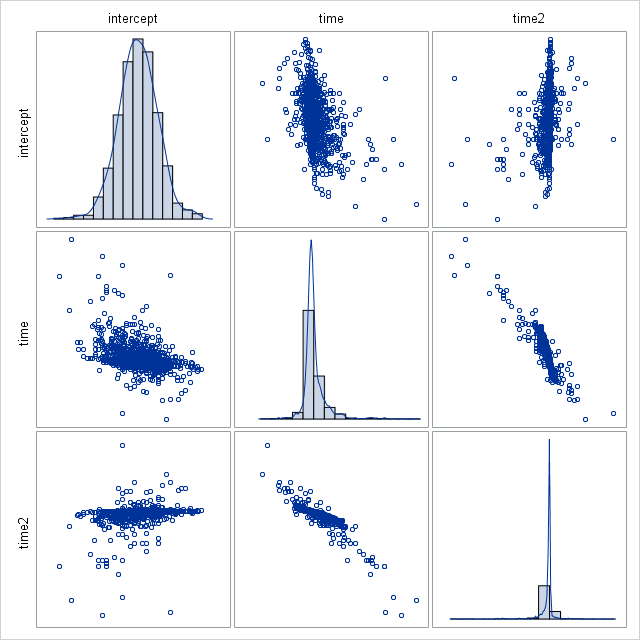
\includegraphics[scale=0.38]{SGScatter2Stage-model.png}
		\caption{Scatter plot for 2 Stage model}
	\end{minipage}
	%\hfill
	\begin{minipage}{.4\textwidth}
		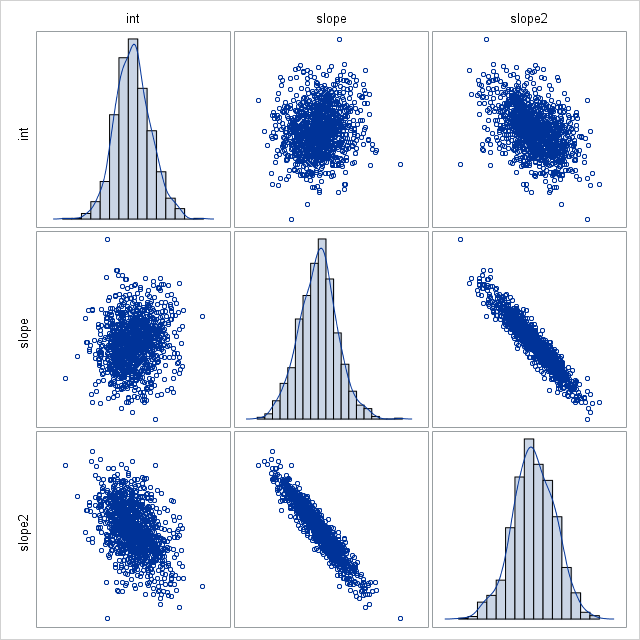
\includegraphics[scale=0.38]{SGScatterRandom-effect.png}
		\caption{Scatter plot for Random model}
	\end{minipage}
\end{figure}

\section{Conclusions}
Several studies have studied the evolution of haematocrit level under different circumstances and it has been observed that the evolution can be influenced by several factors which majorly includes gender. Findings from this study also remains consistent in that direction as data exploration and analysis of the dataset revealed that the evolution of male and females is quite different while that of males is higher than females. In terms of history of cardiovascular problems, conclusions from the three models shows that there is no significant difference in the evolution of haematocrit level for either group of patients. In the case of patients with rejection symptoms and those without rejection symptoms, the multivariate regression model and 2 stage analysis came to a conclusion of no significant difference in evolution of haematocrit level but the linear mixed model came to a border line conclusion. This seemingly contradictory conclusions is due to the evolution pattern of the two groups.


\begin{thebibliography}{99}
%\bibitem{bib1}Bauer, P. and  Bauer, M. M. (1994). Testing equivalence simultaneously for location and  dispersion of two normally distributed populations.  \textit{Biometrical  Journal} \textbf{36}, 643--660.

\bibitem{bib1} Collins, B. (2015). \textit{Renal Transplantation}, Medscape, [online]. Avaiable at:http://emedicine.medscape.com/article/430128-overviewshowall [Accessed 22 Oct. 2016].

\bibitem{bib2} Davis, Charles Patrick. (2016). \textit{Hematocrit Blood Test}, WebMD, [online]. Avaiable at:http://www.emedicinehealth.com/hematocrit-blood-test.htm [Accessed 23 Oct. 2016].

\bibitem{bib3} Gagnon, DR., Zhang, TJ., Brand FN. and Kannel WB. (1994). \textit{Hematocrit and the risk of cardiovascular disease-the Framingham study: a 34-year follow-up}, American Heart Journal, vol. 127, no. 3, Mar, pp. 674-682.

\bibitem{bib4} Mayo Clinic. (2016). \textit{Hematocrit test}, Mayo Clinic,[online]. Avaiable at:http://www.mayoclinic.org/tests-procedures/hematocrit/home/ovc-20205459 [Accessed 23 Oct. 2016].

\bibitem{bib5} Molenberghs, G. and  Verberke, G. (2005). \textit{Models for Discrete Longitudinal Data}. (Springer Series in Statistics), Springer, New York.

\bibitem{bib6} R Core Team. (2015). \textit{R: A Language and Environment for Statistical Computing}. R Foundation for Statistical Computing, Vienna, Austria. 

\bibitem{bib7} SAS. (2015). \textit{SAS/STAT 9.4 User's Guide}. SAS Institute Inc., Cary NC, USA.

\bibitem{bib8} Verbeke, G. and Molenberghs, G. (2000). \textit{Linear Mixed Models For Longitudinal Data} (Springer Series in Statistics), Springer, New York.

\bibitem{bib9} Yu, Y.,  Bo, Y. and Yun C. (2015). \textit{Blood disorders typically associated with renal transplantation}, Front Cell Developmental Biology, vol. 3, Mar 19.
\end{thebibliography}

\section*{Appendix}

\subsection*{Extra Plots}
\begin{figure}[H]
\centering
\begin{minipage}{.4\textwidth}
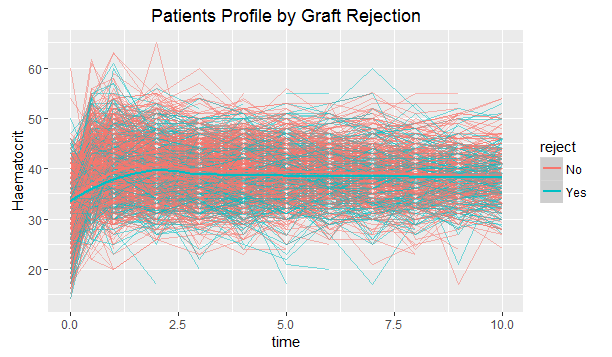
\includegraphics[scale=0.5]{patientprofilegraftrejection.png}
\caption{Profile by Graft Rejection}
\end{minipage}
%\hfill
\begin{minipage}{.5\textwidth}
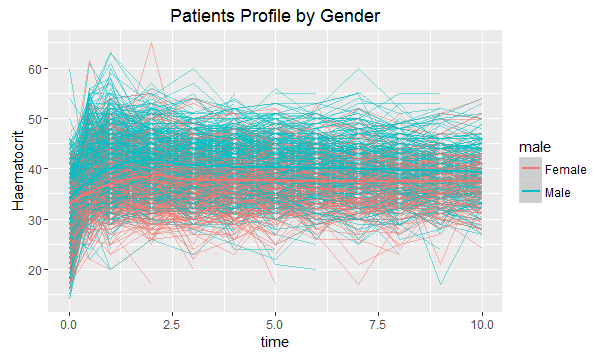
\includegraphics[scale=0.5]{patientsprofilegender.png}
\caption{Profile by Gender}
\end{minipage}
\end{figure}

\begin{figure}[H]
\centering
\begin{minipage}{.5\textwidth}
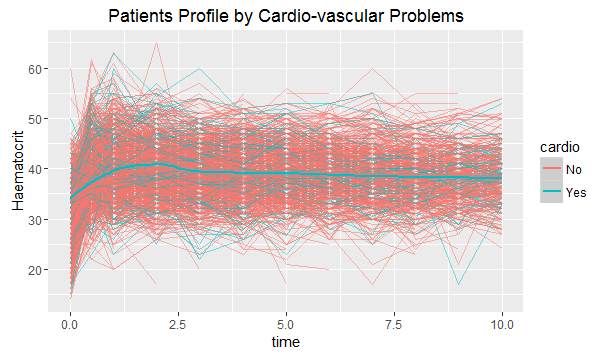
\includegraphics[scale=0.5]{patientprofilecardio.png}
\caption{Profile by Cardio Problems}
\end{minipage}
%\hfill
\begin{minipage}{.4\textwidth}
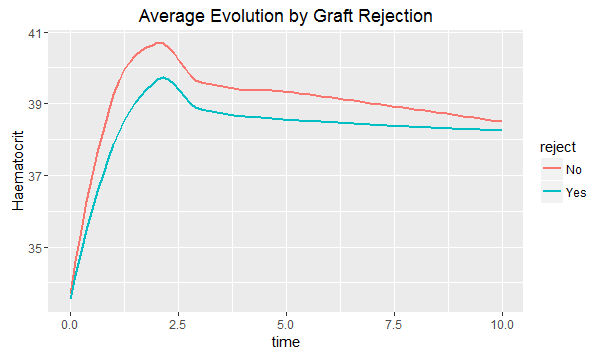
\includegraphics[scale=0.5]{averageevolutionreject.png}
\caption{Evolution by Graft Rejection}
\end{minipage}
\end{figure}

\begin{figure}[H]
\centering
\begin{minipage}{.4\textwidth}

\end{minipage}
%\hfill
\begin{minipage}{.4\textwidth}
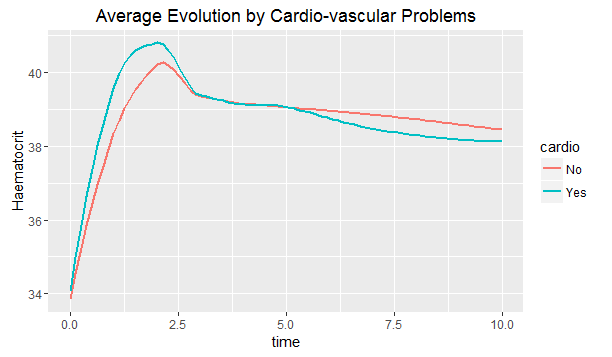
\includegraphics[scale=0.5]{averageevolutioncardio.png}
\caption{Evolution by Cardio}
\end{minipage}
\end{figure}

\begin{figure}[H]
\centering
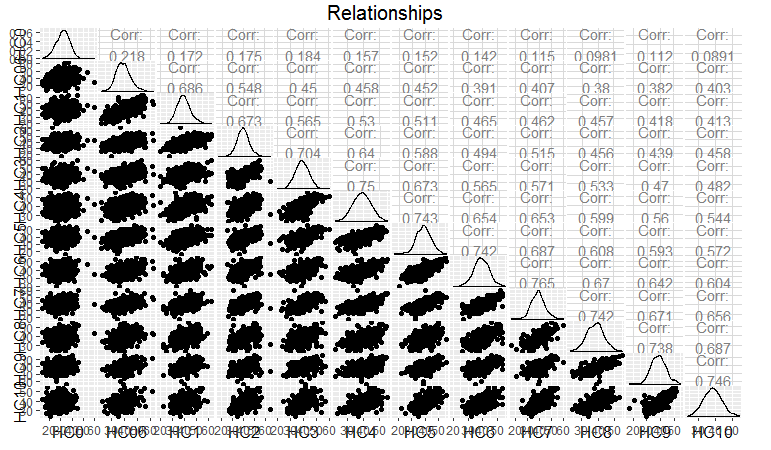
\includegraphics[scale=0.58,width=11cm]{correlationplot.png}
\caption{Correlation Between Timepoints}
\hfill

\end{figure}

\subsection*{Extra Tables}
\begin{table}[H]
\centering
\begin{tabular}{ccccc}
\hline
 & Estimate & SError & t & pvalue\\
 \hline
Intercept & 33.2700 & 0.6206 & 53.61 & $<.0001$\\ 
Age & 0.06261 &  0.009294 & 6.74 & $<.0001$ \\
Male:0 & -1.9124 & 0.2624 & -7.29 & $<.0001$ \\
Cardio:0 & -0.01276 & 0.3587 & -0.04 & 0.9716\\
Reject:0 & 0.3624 & 0.2627 & 1.38 & 0.1681\\
Year & 1.1583 & 0.1439 & 8.05 & $<.0001$\\
Year2 & -0.1192 & 0.008326 & -14.32 & $<.0001$\\
Age*year & 0.001910 & 0.001899 & 1.01 & 0.3149\\
Year*Male:0 & -0.2239 & 0.1234 & -1.81 & 0.0700\\
Year*Cardio:0 & 0.08964 & 0.06554 & 1.37 & 0.1717\\
Year*Reject:0 & -0.06902 & 0.04694 & -1.47 & 0.1418\\
Year2*Male:0 & 0.02473 & 0.01216 & 2.03 & 0.0422\\
\hline
\end{tabular}
\caption{Parameter Estimates of Model 4}
\end{table}

\begin{table}[H]
\centering
\begin{tabular}{ccc}
\hline
 Effect & Mixed Model & Multivariate Model \\
 \hline
%Intercept & 32.2644 & 33.2700  \\ 
%Year & 1.3924 & 1.1583 \\
%$Year^2$ & -0.1451 &  -0.1192 \\
Age & 0.05707 & 0.06261 \\
Male:1 & 34.1623 & 33.2700\\
Cardio:0 & -0.07293 & 31.3576 \\
Reject:1 & -0.2203 & 0.3624 \\
Age*year & 0.000941 & 0.001910\\
Male:1*year & 1.8069 & 1.1583\\
Male:0*year & 1.3924 & 0.9344\\
Cardio:0*year & 0.09646& 0.08964\\
Reject:1*year & -0.2108  & -0.06902\\
Male:1*$year^2$ & -0.1916 & -0.1192\\
Male:0*$year^2$ & -0.1451 & -0.09448\\
Reject:1*$year^2$ & 0.02918  & -\\
\hline
\end{tabular}
\caption{Comparison of Parameter Estimates}
\end{table}

\begin{table}[H]
\centering
\begin{tabular}{cccccc}
\hline
 Effect & Estimate & SError & t & pvalue\\
 \hline
Intercept & 32.2644 & 0.6508  &  49.58  & $<.0001$\\ 
Year & 1.3924 & 0.1532 &9.09  & $<.0001$ \\
$Year^2$ & -0.1451 &  0.01033 & -14.05 & $<.0001$ \\
Age & 0.05707 & 0.009351&   6.10& $<.0001$ \\
Male:1 & 1.8979 & 0.2627 & 7.23 & $<.0001$ \\
Cardio:0 & -0.07293 &  0.3674 &  -0.20 &  0.8426 \\
Reject:1 & -0.2203 & 0.2857 & -0.77 & 0.4407\\
Age*year & 0.000941 &0.001935 & 0.49 & 0.6269\\
Male*year:1 &0.4145 &   0.1257  &  3.30 & 0.0010\\
Cardio*year:0 & 0.09646& 0.06716 & 1.45 &0.1510\\
Reject*year:1 & -0.2108  &   0.1381 & -1.53  &  0.1271\\
$Male*year^2$:1 &-0.04648 &  0.01262& -3.68  & 0.0002\\
$Reject*year^2$:1 & 0.02918  & 0.01368 &  2.13 &  0.0330\\
\hline
\end{tabular}
\caption{Parameter Estimates of the Random-effects model}
\end{table}
\subsection{SAS \& R Codes}
\begin{multicols}{2}
\begin{verbatim}
#reading the data
renaldata <- read_sas
('./Data/renal.sas7bdat')
#creating the long format
renaldata_long <- renaldata %>%
gather(key='time',
value='Haematocrit',-id,-age,
-male,-cardio,-reject)
#cleaning the time variable
renaldata_long <- renaldata_long %>%
mutate(time=gsub('HC','',time))
#to avoid 06 becoming 6, 
#it is recoded as 0.5
renaldata_long <- renaldata_long %>%
mutate(time
=as.numeric(gsub('06','0.5',time)))
#creating quadratic time
renaldata_long <- renaldata_long
%>% mutate(time2=time^2)
renaldata$cardio <- factor(renaldata
$cardio,
labels = c('No','Yes'))
renaldata$reject <- factor(renaldata
$reject,
labels = c('No','Yes'))
renaldata$male <- factor(renaldata
$male,
labels = c('Female','Male'))
#Some summaries
renalmean <- renaldata_long %>% 
group_by(time) %>%
summarise(averagemeasure=
mean(Haematocrit,na.rm=T),
variance=var(Haematocrit,na.rm=T),
nummeasure=sum(!is.na(Haematocrit)))
###Missing pattern
missingpattern <- function(x){
  y <- NULL
    for(i in 1:nrow(x)){
      a <- is.na(x[i,])
      a[a==T] <- 'X'
      a[a==F] <- '-'
      y[i] <- paste0(a,collapse='')
    }
  return(y)
}
renaldata$mpattern <- 
missingpattern(
renaldata %>% dplyr::select
(HC0,HC06,HC1,HC2,HC3,
HC4,HC5,HC6,HC7,HC8,HC9,HC10))
table(renaldata$mpattern)
#patients profile
renaldata_long %>% 
ggplot(aes(x=time,y=
Haematocrit)) + 
geom_point(alpha=0.1,col=2) + 
geom_line(aes(group=id),
alpha=0.3,col=1) + 
ggtitle('Individual 
Patients profile')
+ geom_smooth(se=F,
method =
'loess',col=2)
renaldata_long %>% 
ggplot(aes(x=time,y=Haematocrit)) +
ggtitle(' Average 
Haematocrit Evolution') + 
geom_smooth(se=F,
method = 'loess',col=2)
#patients profile by gender
renaldata_long$male <- 
factor(renaldata_
long$male,
labels = 
c('Female','Male'))
renaldata_long %>% 
ggplot(aes(x=time,
y=Haematocrit,colour=male)) 
+ geom_point(alpha=0.6) + 
geom_line(aes(group=id)
,alpha=0.5) + 
ggtitle('Patients 
Profile by Gender') +
geom_smooth(method = 'loess')
#mean structure by cardio
renaldata_long %>%
ggplot(aes(x=time,
y=Haematocrit,colour=cardio))
+ geom_smooth(method = 
'loess',se=F) + 
ggtitle('Average Evolution
by Cardio-vascular Problems')
#mean structure by graft
renaldata_long %>%
ggplot(aes(x=time,
y=Haematocrit,
colour=reject)) + 
geom_smooth(method = 
'loess',se=F) + 
ggtitle('Average
Evolution by 
Graft Rejection')
#variance components
renaldata_long %>%
ggplot(aes(x=factor(time)
,y=Haematocrit))
+ geom_jitter()
renaldata_long %>%
ggplot(aes(x=factor(time)
,y=Haematocrit))+
geom_boxplot() + 
ggtitle('Variance 
Function') + 
labs(x='time')
#correlation structure
ggpairs(renaldata[,1:12]
,title='Relationships')
resids2 <- as.numeric((loess(
Haematocrit~time,
data=renaldata_long)
$residuals)^2)
x <-
as.numeric(
loess(Haematocrit~time
,data=renaldata_long)$x)
plotdata <- tibble(x
,resids2)
ggplot(plotdata,
aes(x,resids2,
colour=renaldata_
long$male)) + 
geom_point() + 
geom_smooth(method=
'loess',se=F) + 
labs(x='time',
y='Squared Residuals') +
ggtitle('Smoothed 
Variance Function')
# Two stage analysis
#regression model)
#simple regression
r2 <- numeric(1160)
sse2i <- 
numeric(1160)
ssr2i <- 
numeric(1160)
ni <- 
numeric(1160)
pi <- 
numeric(1160)
interceptlin <- 
numeric(1160)
slopelin <- 
numeric(1160)
seint <- 
numeric(1160)
seslope <- 
numeric(1160)
for(i in 1:1160){
  mod <-
  lm(Haematocrit~time,
  data=renaldata_
  long[(renaldata_
  long$id==i),],x=T)
  r2[[i]] <- 
  summary(mod)$
  r.squared
  sse2i[[i]] <- 
  sum(mod$residuals^2)
  ssr2i[[i]] <- 
  anova(mod)$
  `Sum Sq`[[1]]
  ni[[i]] <- 
  length(mod$x[,1])
  pi <- 
  length(mod$
  coefficients)
  interceptlin[[i]] 
  <- 
  mod$coefficients[[1]]
  slopelin[[i]] <- 
  mod$coefficients[[2]]
  seint[[i]] <-
  summary(mod)$
  coefficients[,2][1]
  seslope[[i]] <- summary(mod)
  $coefficients[,2][2]
}
lineardata <-
tibble(r2,sse2i,
ssr2i,ni,pi,interceptlin,
slopelin,seslope,seint)
r2metalinear <-
sum(lineardata$ssr2i)
/sum(lineardata$ssr2i+
lineardata$sse2i)
#quadratic 
r2q <- 
numeric(1160)
sse2qi <- 
numeric(1160)
ssr2qi <- 
numeric(1160)
nqi <- 
numeric(1160)
pqi <- 
numeric(1160)
interceptquad <- 
numeric(1160)
slopequad <- 
numeric(1160)
slopequad2 <- 
numeric(1160)
quadseint <- 
numeric(1160)
quadseslope1 <- 
numeric(1160)
quadseslope2 <- 
numeric(1160)

for(i in 1:1160){
  mod <- lm(Haematocrit~time
  +time2,
  data=renaldata_
  long[(renaldata_
  long$id==i),],x=T)
  r2q[[i]] <-
  summary(mod)
  $r.squared
  sse2qi[[i]] <-
  sum(mod$residuals^2)
  ssr2qi[[i]] <- 
  anova(mod)$
  `Sum Sq`[[1]]
  nqi[[i]] <- 
  length(mod$x[,1])
  pqi <- 
  length(mod$
  coefficients)
  interceptquad[[i]] <- 
  mod$coefficients[[1]]
  slopequad[[i]] <- 
  mod$coefficients[[2]]
  slopequad2[[i]] <- mod
  $coefficients[[3]]
  quadseint[[i]] <- summary(mod)
  $coefficients[,2][1]
  quadseslope1[[i]] <- summary(mod)
  $coefficients[,2][2]
  quadseslope2[[i]] <- summary(mod)
  $coefficients[,2][3]
}
quadraticdata <-
tibble(r2q,sse2qi,ssr2qi,
nqi,pqi,interceptquad,
slopequad,slopequad2,
quadseint,quadseslope1
,quadseslope2)
#r2 meta
r2metaquadratic <- 
sum(quadraticdata$ssr2qi)/
sum(quadraticdata$ssr2qi
+quadraticdata$sse2qi)
##computing Fmeta
pstar <- lineardata$pi
ppstar <- quadraticdata$pqi
t <- pstar + ppstar
t2 <- ppstar - pstar

Fmeta <- (sum(lineardata$sse2i
[lineardata$ni 
>= t] - 
quadraticdata$
sse2qi[lineardata$ni >= t])/
sum(t2[lineardata$ni >= t])) /
(sum(quadraticdata$sse2qi
[lineardata$ni >= t])/
sum(lineardata$ni
[lineardata$ni >= 
t] - 
ppstar[lineardata$ni >= t]))

(sum(lineardata$sse2i - 
quadraticdata$sse2qi)/
sum(pstar)) / 
(sum(quadraticdata$sse2qi)/
sum(lineardata$ni - t))

#pval fmeta
pf(Fmeta,sum(t2[lineardata$ni >=
t]),sum(lineardata$
ni[lineardata$ni >= t]
- ppstar[lineardata$ni 
>= t]),lower.tail = F)
#2nd stage
modelint <- 
lm(quadraticdata$
interceptquad~
renaldata$age+
renaldata$male+
renaldata$cardio+
renaldata$reject,
weights = quadraticdata$quadseint)
#using linear time slope
modelint2 <-
lm(quadraticdata$
slopequad~renaldata$age+
renaldata$male+
renaldata$cardio+
renaldata$reject,
weights = 
quadraticdata$quadseslope1)
#using quadratic time slope
modelint3 <-
lm(quadraticdata$
slopequad2~renaldata$age+
renaldata$male+renaldata$
cardio+renaldata$reject,
weights = quadraticdata$quadseslope2)
#####SAS
*Multivariate model-final model;
proc mixed data=Tmp1.renal5 
method=ml;
class id male cardio 
reject yearcss;
model Hc = year year2 
age male cardio reject
age*year male*year 
cardio*year 
reject*year 
male*year2 / s;
repeated  yearcss
/ type=un subject=id;
run; 
*Random-effect model-final model;
proc mixed 
data=Tmp1.renal5
order=data 
method=reml 
covtest empirical;
class male 
cardio reject
yearcss;
model Hc = year year2
age male cardio
reject age*year male*year
cardio*year 
reject*year male*year2 
reject*year2/ s;
random intercept 
year year2 /
type=un subject=id 
g gcorr v vcorr solution;
ods listing 
exclude solutionr;
ods output 
solutionr=out;
repeated yearcss/ 
type=simple subject=id;
run;
*contrast for 
male vs female;
proc mixed 
data=Tmp1.renal5 method=ml;
class id male 
cardio reject yearcss;
model Hc = age 
male cardio reject 
age*year male*year 
cardio*year reject*year 
male*year2/ ddfm=satterth noint s;
contrast 'Evolution of 
Males vs Females' male 1 -1,
male*year 1 -1,
male*year2 1 -1 /chisq;
repeated yearcss/
type=un subject=id;
run;
*contrast for 
cardio0 vs cardio0;
proc mixed 
data=Tmp1.renal5
method=ml;
class id male 
cardio reject yearcss;
model Hc= age male 
cardio reject 
age*year male*year 
cardio*year reject*year 
male*year2/ ddfm=satterth noint s;
contrast 'Evolution of 
Cardio vs No Cardio' cardio 1 -1,
cardio*year 1 -1 /chisq;
repeated yearcss/
type=un subject=id;
run;
*contrast for
reject0 vs reject1;
proc mixed 
data=Tmp1.renal5 
method=ml;
class id male cardio 
reject yearcss;
model Hc = age male 
cardio reject age*year 
male*year cardio*year 
reject*year 
male*year2/ 
ddfm=satterth noint s;
contrast 'Evolution of 
Reject vs 
No Reject' 
reject 1 -1,
reject*year 
1 -1 /chisq;
repeated 
yearcss/type=un 
subject=id;
run;

\end{verbatim}

\end{multicols}

\end{document}
